% !TeX spellcheck = de_DE
%%% Ne pas modifier jusqu'à la ligne 25
\documentclass[a4paper,14pt,UTF8]{article}
\usepackage[utf8]{inputenc}
\usepackage[french]{babel}
\usepackage[left=2cm,right=2cm,top=3cm,bottom=2cm, headheight=1.5cm,headsep=1.5cm]{geometry}

\usepackage{palatino}
\usepackage{setspace}
\usepackage{caption}
\usepackage{float}%控制浮动体位置
%设置段落之间的距离,若不需要删除或者注释掉即可。
\usepackage{blindtext}
\usepackage{fancyhdr}
\usepackage{xcolor} % 代码高亮

\usepackage{mathrsfs}
\usepackage{amsmath,amsfonts,amssymb,dsfont}
\usepackage{graphicx}
\usepackage{enumitem}		%\enumerate-resume
\usepackage[colorlinks=true,unicode={true},hyperindex=false, linkcolor=black, urlcolor=black]{hyperref}
\usepackage{lastpage} 
\usepackage{ctex}			% 中文
\usepackage{comment}		% 注释大段代码
\usepackage{pifont}			% 列表环境

%\renewcommand\thesection{\Roman{section}~-~}
%\renewcommand\thesubsection{\Roman{section}.\Alph{subsection}~-~}
%\renewcommand\thesubsubsection{\Roman{section}.\Alph{subsection}.\arabic{subsubsection}~-~}
\renewcommand\thesection{\arabic {section}}


\setcounter{secnumdepth}{3}
\parindent=0pt

\usepackage{fancyhdr}
\pagestyle{fancy}

\lhead{SJTU-ParisTech}
%%%%%%%%%%%%%%%%%%%%%%%%%%%%%%%
\chead{PLT -- Compilateur d'automate}
\rhead{page \thepage\ de \pageref{LastPage}} % 当前页 of 总页数

\begin{document}
	
	\renewcommand{\labelitemi}{$\blacktriangleright$}
	\renewcommand{\labelitemii}{$\bullet$}
	
	\linespread{1.15}
	\selectfont
	\setlength{\parskip}{0.5em}
	
	
	%%% Page de garde
	\thispagestyle{empty}
	\begin{center}
		
\includegraphics{cover5}
		\hspace{60pt}
		
\includegraphics{cover2}
	\end{center}
	%
	\vspace{125pt}
	%
	\begin{center}
		\scalebox{1.3}{\LARGE{\textbf{Théorie des Langages de Programmation}}}

	\end{center}
	%
	\vspace{2em} \Large
	%
	\begin{center}
		\textbf{Henri \quad 516261910008}

	\end{center}
	%
	\vspace{1em}
	%
	\begin{center}
		
\includegraphics[scale=1.2]{cover3}
	\end{center}
	%
	\vspace{1em} \normalsize
	%

	
	\newpage
	\begin{center}
		\tableofcontents
	\end{center}
	\numberwithin{equation}{section}
	\clearpage
	
	\section{Introduction}
	\quad Les codes sont écrits dans VScode (langue C) et exécutés sur linux. J'ai vérifié \ bien qu'il n'y a ni erreur ni warning pour la compilation.
	Les variables sont nommées en anglais mais tous les commentaires sont écrits en français.	Les fichers \textit{*.c} sont les fichers avec \textit{main function} à \ tester, et les fichiers \textit{*.h} contiennent les définitions des fonctions. 
	
	\begin{figure}[h]
		\setlength{\abovecaptionskip}{-0.cm}
		
		\begin{center}
			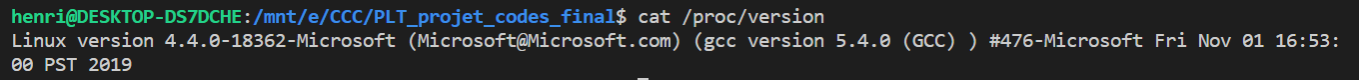
\includegraphics[width=17cm]{1_env}
		\end{center}
		\caption{Environnement de la compilation et l'exécution}
	\end{figure}
	
	\quad Pour les parties \textit{analyse lexicale}, \textit{analyse syntaxiaue} et \textit{analyse sémantique}, je donne un bon exemple et un exemple avec des érreurs pour tester. $(i.e. Dpile.txt, Test- lexical.txt, Test-syntaxique.txt, Test-semantique.txt)$ Après avoir fini ces trois analyses, j'ai réalisé \ une compilation afin d'obtenir la machine virtuelle. Finalement, selon cette machine virtuelle, j'examine si l'une expression est acceptée ou refusée.
	
	
	
	\section{Diagramme du système}
	\quad On veut écrire un compilateur d'automate qui lit un fichier contenant la description de l'automate et produit en machine virtuelle un code capable de reconnaître ou pas tout mot qui lui sera fourni. Il permet aussi
	d'exécuter les machines virtuelles écrites. 
	
	\quad L'analyse lexical donne le lexème de l'automate. Puis, l'analyse syntaxique prend ce lexème, examine le syntaxe et donne un arbre syntaxique. Ensuite, l'analyse sémantique prend cet arbre syntaxique, vérifie qu'il a du sens et donne un arbre syntaxique correct. On fait la compilation selon cet arbre et obtient une machine virtuelle. Enfin, on réalise l'exécution selon cette machine virtuelle et vérifie si le mot donné \ est valid ou invalid.
	
	\begin{figure}[h]
		\setlength{\abovecaptionskip}{-0.cm}
		
	\begin{center}
		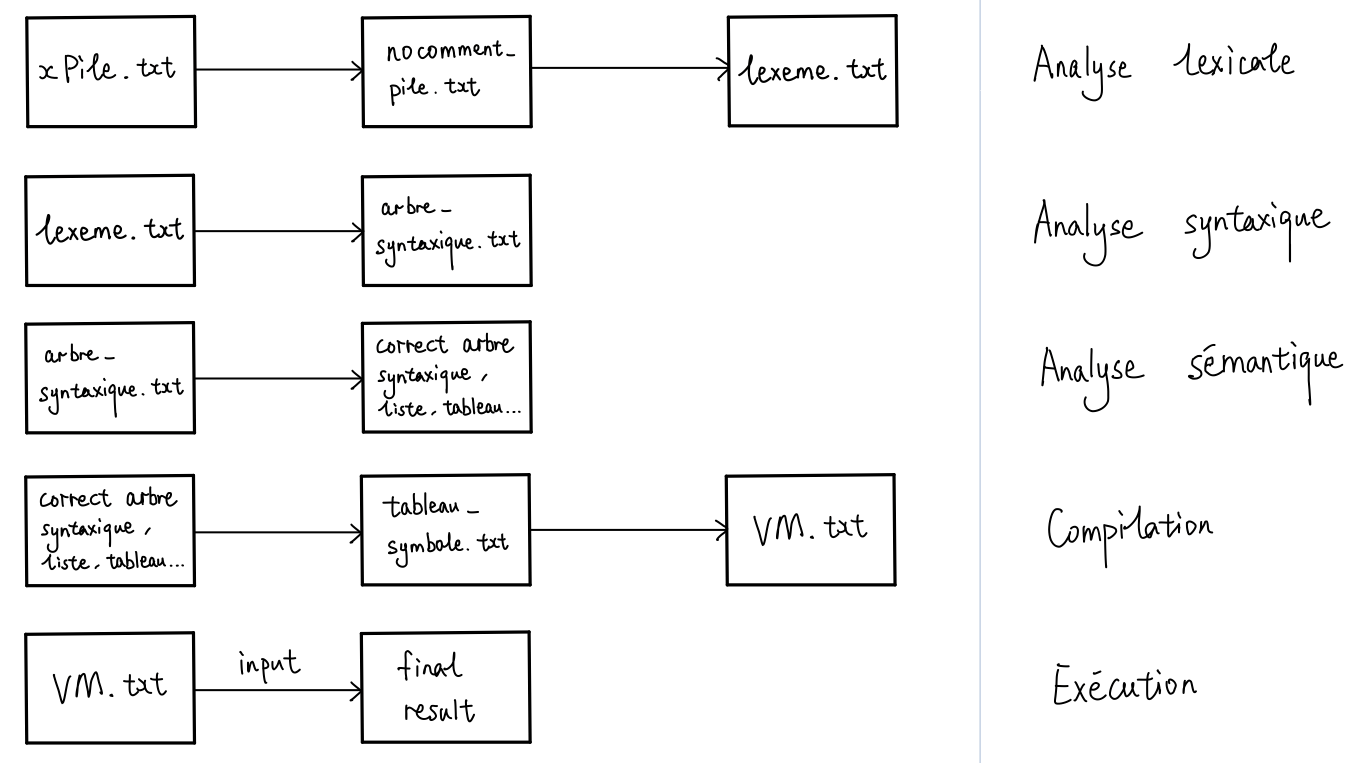
\includegraphics[width=16cm]{system_diagram}
	\end{center}
		\caption{Le diagramme de la programmation}
	\end{figure}
	

	\section{Description des fonctions}
	
	\subsection{\textit{analyse lexicale}}
	\quad Dans cette partie, les deux fichiers concernés sont \textit{analyseur-lexical.c} et \textit{analyseur-lexical.h}. Le *.c fichier contient la \textit{main function} et le *.h fichier contient les définitions des fonctions utilisées. Les deux fichiers pour tester sont \textit{Dpile.txt} et \textit{Test-lexical.txt}. Si on détecte les erreurs, le programme s'arrête et donne le type des erreurs.  \par 


	\begin{itemize}
		
	\item 
	Fonction \textit{supprimer-commentaire} a pour but de supprimer les commentaires dans le fichier donné. Par exemple, les paragraphes entre ${\rm{/*}} \ ... \ {\rm{*/}}$ ou les lignes apès ${\rm{//}}... \ $ sont les commentaires à \ enlever. J'ai appliqué \ un automate avec 5 états pour réalisé \  cette fonction. L'entrée de cette fonction est le fichier donné, et la sortie est le fichier \textit{nocomment.txt}.
	
	\begin{figure}[H]
		\setlength{\abovecaptionskip}{-0.cm}
		
		\begin{center}
			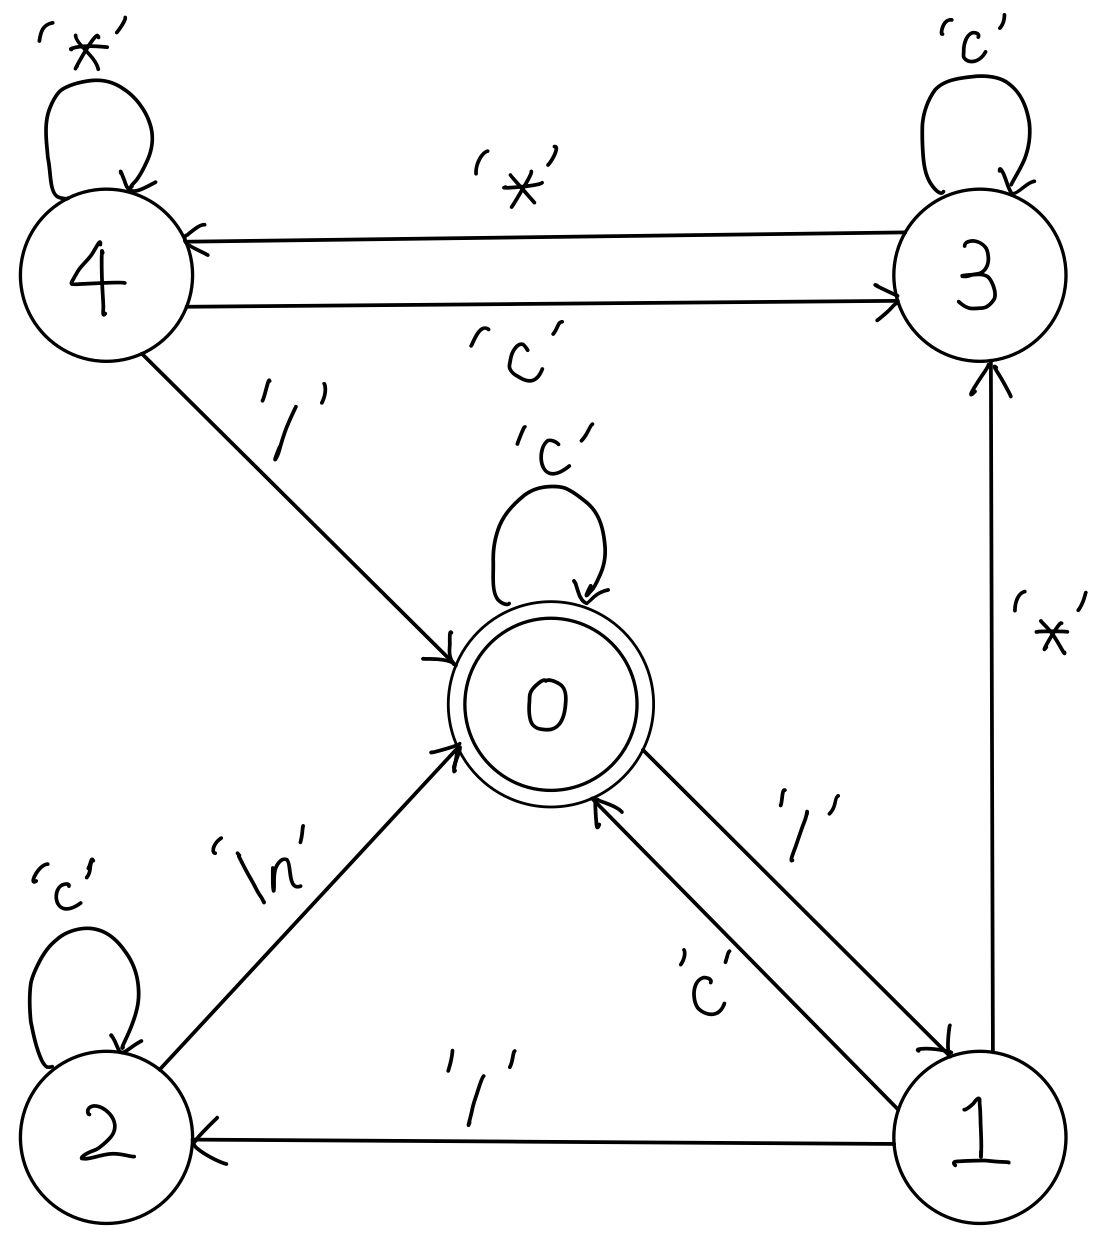
\includegraphics[width=7cm]{supprimer_commentaire}
		\end{center}
		\caption{L'automate avec 5 états pour supprimer les commtaires}
	\end{figure}
	
	\item
	Fonction \textit{traiter-file} est définie pour supprimer les espaces et les newlines dans le fichier \textit{nocomment.txt}. La sortie de cette fonction est le fichier \textit{lexeme.txt}. \\
	
	\item
	Fonction \textit{examiner-caracteres} est utilisée pour vérifier si tous les caractères (lettre par lettre) dans le fichier \textit{lexeme.txt} sont valides (dans le lexème que je définis)) ou pas. Si non, le fichier est lexicalement faux et on arrête le programme.
	
	\begin{figure}[H]
		\setlength{\abovecaptionskip}{-0.cm}
		
		\begin{center}
			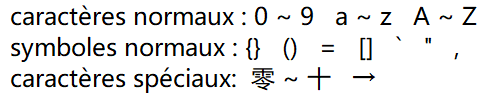
\includegraphics[width=8cm]{lexeme}
		\end{center}
		\caption{Lexème de l'automate}
	\end{figure}
	
	\item
	Fonction \textit{examiner-mots} est dans le but de vérifier si les mots dans le fichier \textit{lexeme.txt} sont des mots clés. C'est à \ dire que
	les 5 mots français : \textbf{Automate, etats, initial, final, transitions}.
	Si non, le fichier contient des mots invalids. Alors, le fichier est lexicalement faux et on arrête le programme. Si le fichier \textit{lexeme.txt} passe ces deux fonctions sans avoir d'erreur, alors on obtient le lexème de l'automate donné.
	
	\end{itemize}
	
		  
	\subsection{\textit{analyse syntaxique}}
	\quad Dans cette partie, les deux fichiers concernés sont \textit{analyseur-syntaxique.c} et \textit{analyseur-syntaxique.h}. Le *.c fichier contient la \textit{main function} et le *.h fichier contient les définitions des fonctions utilisées. Les deux fichiers pour tester sont \textit{Dpile.txt} et \textit{Test-syntaxique.txt}. Si on détecte les erreurs, le programme s'arrête et donne le type des erreurs. \par 

	
	\begin{itemize}
		
		\item 
		Function \textit{examiner-syntaxique} réalise l'analyse syntaxique en appliquant un automate avec 50 états. Cet automate restreint la formule du fichier de l'automate exactement comme les trois exemples. Par exemple, le premier mot doit être Automate, suivant les deux crochets et le nombre de piles, puis la signe d'égalité, etc. On limite l'écriture du fichier strictement. Tant qu'il y a une erreur du grammaire ou du syntaxe, le fichier est syntaxiquement faux et on arrête le programme. 
		
		\begin{figure}[H]
			\setlength{\abovecaptionskip}{-0.cm}
			
			\begin{center}
				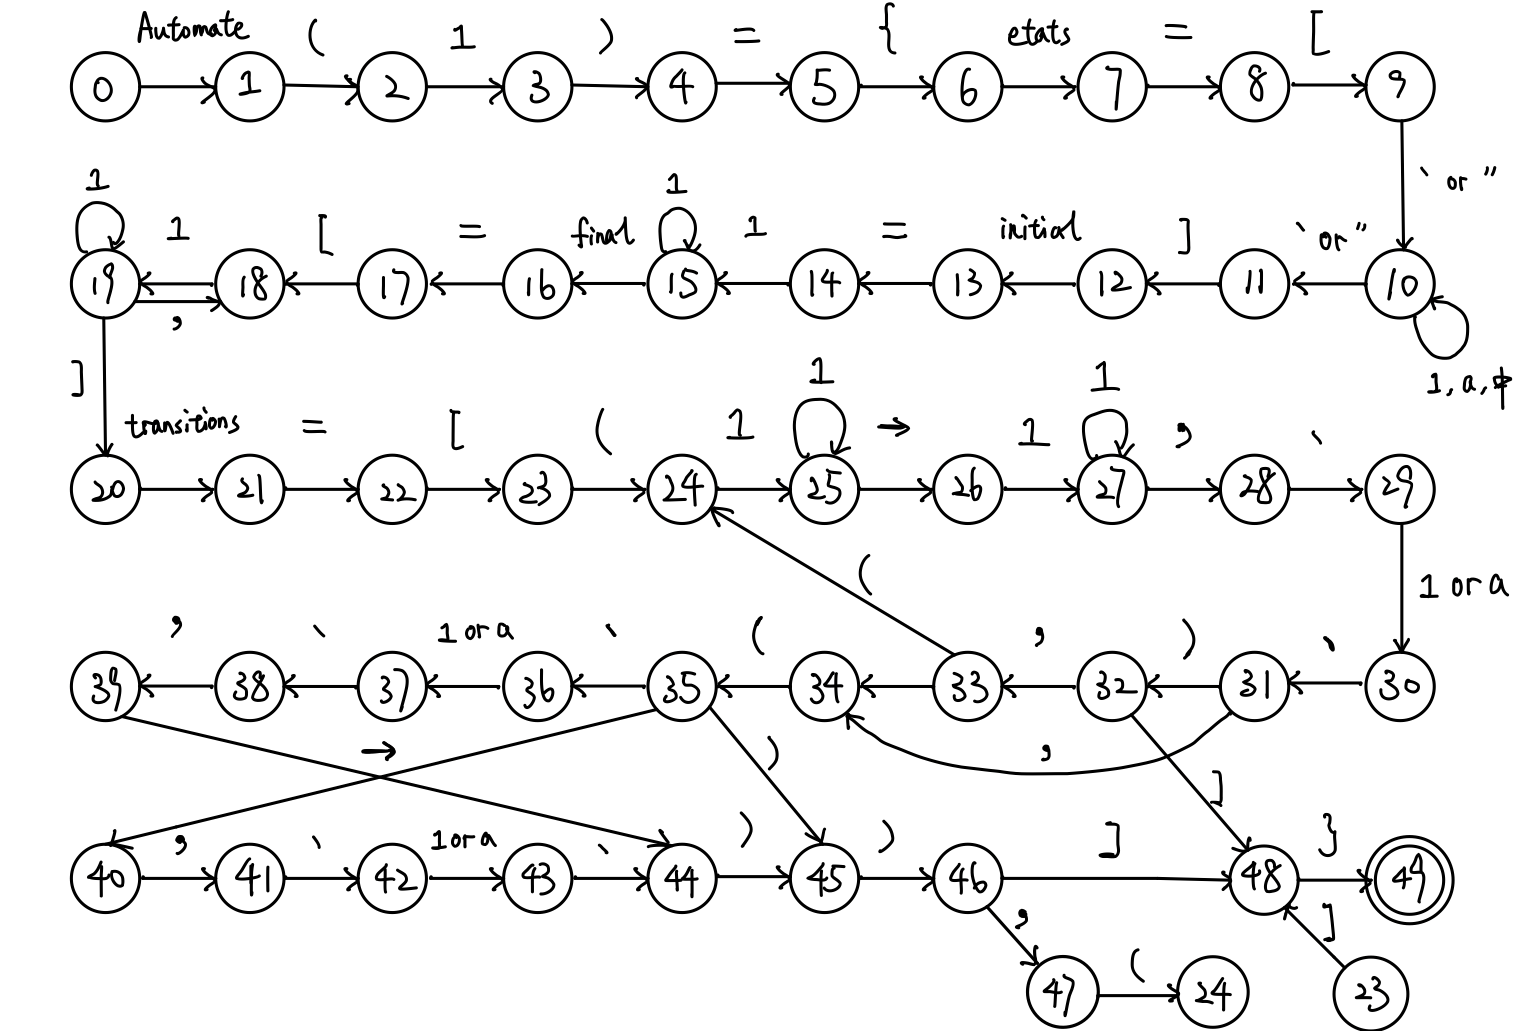
\includegraphics[width=16cm]{analyse_syntaxique}
			\end{center}
			\caption{L'automate avec 50 états pour réaliser l'analyse syntaxique}
		\end{figure}
		
		
		\item 
		La grammaire BNF de mon automate est définie comme suivante: 
		
			\begin{description}
				
				\item[\ding{47}] \textless lettre\textgreater ::= ``a" $|$ ... $|$ ``z" $|$ ``A" $|$ ... $|$ ``Z" \par
				
				\item[\ding{47}] \textless chiffre\textgreater ::= ``0" $|$ ... $|$ ``9" \par
				
				\item[\ding{47}] \textless naturel\textgreater ::= \textless chiffre\textgreater  $\lbrace$\textless chiffre\textgreater $\rbrace$\par
				
				\item[\ding{47}] \textless naturels\textgreater ::= $\lbrace$\textless naturel\textgreater ``,"$\rbrace$ \textless naturel\textgreater \par
				
				\item[\ding{47}] \textless guillemet\textgreater ::= `` ` " $|$ `` " " \par
				
				\item[\ding{47}] \textless chinois\textgreater ::= ``零" $|$ ``一" $|$ ``二" $|$ ``三" $|$ ``四" $|$ ``五" $|$ ``六" $|$ ``七" $|$ ``八" $|$ ``九" $|$ ``十"
				
				\item[\ding{47}] \textless spécial\textgreater ::= \textless chinois\textgreater \ $|$ ``$ \to$" \par
				
				\item[\ding{47}] \textless début\textgreater ::= ``Automate=(" ``0"$|$``1"$|$``2" ``)" \par
				
				\item[\ding{47}] \textless initial\textgreater ::= ``initial="\textless naturel\textgreater \par
				
				\item[\ding{47}] \textless mot\textgreater ::= \textless lettre\textgreater  \ $|$ \textless lettre\textgreater \textless mot\textgreater \par
				
				\item[\ding{47}] \textless état\textgreater ::= \textless guillemet\textgreater (\textless naturel\textgreater$|$\textless mot \textgreater$|$\textless chinois\textgreater)\textless guillemet\textgreater \par
				
				\item[\ding{47}] \textless états\textgreater ::= $\lbrace$\textless etats\textgreater``,"$\rbrace$ \textless etat\textgreater
				
				\item[\ding{47}] \textless élément\textgreater ::= \textless guillemet\textgreater (\textless chiffre\textgreater $|$\textless lettre\textgreater)\textless guillemet\textgreater \par
				
				\item[\ding{47}] \textless push\textgreater ::= `` ($\to$, "\textless élément\textgreater   ``)''\par
				
				\item[\ding{47}] \textless pop\textgreater ::= ``("\textless élément\textgreater  ``, $\to$)" \par
				
				\item[\ding{47}] \textless trans\textgreater ::= \textless naturel\textgreater ``$\to$"\textless naturel\textgreater ``,"\textless guillemet\textgreater \textless élément\textgreater \textless guillemet\textgreater \par
				
				\item[\ding{47}] \textless pile\textgreater ::= ``,"( \textless push\textgreater \ $|$ \textless pop\textgreater \ $|$ ``()" ) \par
				
				\item[\ding{47}] \textless transition\textgreater ::= ``(" ( \textless trans\textgreater \ $|$ \textless trans\textgreater \textless pile\textgreater \ $|$ \textless trans\textgreater \textless pile\textgreater \textless pile\textgreater ) ``)" \par
				
				\item[\ding{47}] \textless transitions\textgreater ::= $\lbrace$\textless transition\textgreater ``,"$\rbrace$ \textless transition\textgreater \par
				
				\item[\ding{47}] \textless expr\textgreater ::= ( (``états"$|$``final"$|$``transitions") ``=["\textless naturels\textgreater $|$\textless états\textgreater $|$\textless transitions\textgreater ``]" ) $|$ \textless initial\textgreater \par
				
				\item[\ding{47}] \textless exprs\textgreater ::= $\lbrace$\textless expr\textgreater$\rbrace$ \par
				
				\item[\ding{47}] \textless automate\textgreater ::= \textless début\textgreater ``$\lbrace$"\textless exprs\textgreater  ``$\rbrace$" \par

			\end{description}
		
		\begin{comment}
			\begin{flushleft}
			$\bullet$ \textless lettre\textgreater ::= ``a" $|$ ... $|$ ``z" $|$ ``A" $|$ ... $|$ ``Z" \par 
			
			$\bullet$ \textless chiffre\textgreater ::= ``0" $|$ ... $|$ ``9" \par
			
			$\bullet$ \textless naturel\textgreater ::= \textless chiffre\textgreater  $\lbrace$\textless chiffre\textgreater $\rbrace$\par
			
			$\bullet$ \textless naturels\textgreater ::= $\lbrace$\textless naturel\textgreater ``,"$\rbrace$ \textless naturel\textgreater \par
			
			$\bullet$ \textless guillemet\textgreater ::= `` ` " $|$ `` " " \par
			
			$\bullet$ \textless chinois\textgreater ::= ``零" $|$ ``一" $|$ ``二" $|$ ``三" $|$ ``四" $|$ ``五" $|$ ``六" $|$ ``七" $|$ ``八" $|$ ``九" $|$ ``十"
			
			$\bullet$ \textless spécial\textgreater ::= \textless chinois\textgreater \ $|$ ``$ \to$" \par
			
			$\bullet$ \textless début\textgreater ::= ``Automate=(" ``0"$|$``1"$|$``2" ``)" \par
												
			$\bullet$ \textless initial\textgreater ::= ``initial="\textless naturel\textgreater \par
		
			$\bullet$ \textless mot\textgreater ::= \textless lettre\textgreater  \ $|$ \textless lettre\textgreater \textless mot\textgreater \par
			
			$\bullet$ \textless état\textgreater ::= \textless guillemet\textgreater (\textless naturel\textgreater$|$\textless mot \textgreater$|$\textless chinois\textgreater)\textless guillemet\textgreater \par
			
			$\bullet$ \textless états\textgreater ::= $\lbrace$\textless etats\textgreater``,"$\rbrace$ \textless etat\textgreater

			
			$\bullet$ \textless élément\textgreater ::= \textless guillemet\textgreater (\textless chiffre\textgreater $|$\textless lettre\textgreater)\textless guillemet\textgreater \par
			
			$\bullet$ \textless push\textgreater ::= `` ($\to$, "\textless élément\textgreater   ``)''\par
			
			$\bullet$ \textless pop\textgreater ::= ``("\textless élément\textgreater  ``, $\to$)" \par
			
			$\bullet$ \textless trans\textgreater ::= \textless naturel\textgreater ``$\to$"\textless naturel\textgreater ``,"\textless guillemet\textgreater \textless élément\textgreater \textless guillemet\textgreater \par
			
			$\bullet$ \textless pile\textgreater ::= ``,"\textless push\textgreater \ $|$ \textless pop\textgreater \ $|$ ``()" \par
			
			$\bullet$ \textless transition\textgreater ::= ``("\textless trans\textgreater \ $|$ \textless trans\textgreater \textless pile\textgreater \ $|$ \textless trans\textgreater \textless pile\textgreater \textless pile\textgreater ``)" \par
			
			$\bullet$ \textless transitions\textgreater ::= $\lbrace$\textless transition\textgreater ``,"$\rbrace$ \textless transition\textgreater \par
			
			$\bullet$ \textless expr\textgreater ::= ( (``états"$|$``final"$|$``transitions") ``=["\textless naturels\textgreater $|$\textless états\textgreater $|$\textless transitions\textgreater ``]" ) $|$ \textless initial\textgreater \par
			
			$\bullet$ \textless exprs\textgreater ::= $\lbrace$\textless expr\textgreater$\rbrace$ \par
			
			$\bullet$ \textless automate\textgreater ::= \textless début\textgreater ``$\lbrace$"\textless exprs\textgreater  ``$\rbrace$" \par
			
			\end{flushleft}
		\end{comment}
		
		\vspace{2pt}
		
		\item 
		L'entrée de cette fonction est \textit{lexeme.txt} et la sortie est le fichier \textit{arbre-syntaxique.txt}. Selon ce fichier, on produit le graphe de l'arbre syntaxique par graphviz. Cet arbre montre les informations importantes et la structure de l'automate. \par
		
		\par
		
		\begin{figure}[H]
			\setlength{\abovecaptionskip}{-0.cm}
			
			\begin{center}
				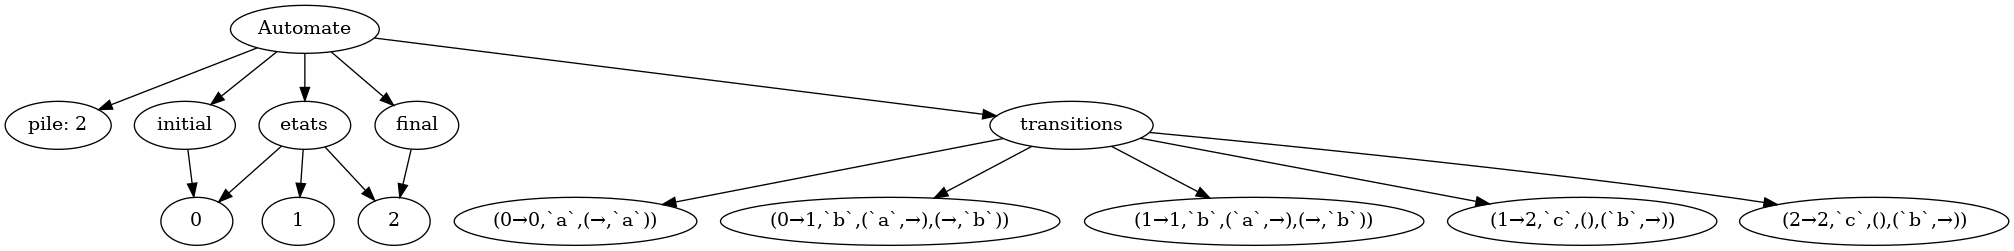
\includegraphics[width=16cm]{arbre_syntaxique}
			\end{center}
			\caption{Un exemple de l'arbre syntaxique}
		\end{figure}
		
	\end{itemize} 
   
	\subsection{\textit{analyse sémantique}}
	
	\quad Dans cette partie, les deux fichiers concernés sont \textit{analyseur-semantique.c} et \textit{analyseur-semantique.h}. Le *.c fichier contient la \textit{main function} et le *.h fichier contient les définitions des fonctions utilisées. Les deux fichiers pour tester sont \textit{Dpile.txt} et \textit{Test-semantique.txt}. Si on détecte les erreurs, le programme s'arrête et donne le type des erreurs.  \par 

	
	\begin{itemize}
		
		\item 
		Fonction \textit{examiner-arbre-syntaxique} est la fonction définie pour vérifier que l'arbre syntaxique que l'on a obtenu a du sens. Je vérifie les points suivants : \par
		
			\begin{description}
				
				\item[\ding{47}] Mots clés sont tous là. \ (\textbf{Automate, etats, initial, final, transitions})\par
				
				\item[\ding{47}] ll n'y pas de répétition dans l'état. \ (ex. etats = [一, 一, 二, 三])\par
				
				\item[\ding{47}] Les numéros des états, de l'initial et du final ne dépassent pas le nombre de l'état moins un.\par
				
				\item[\ding{47}] Les numéros des états dans les transitions ne dépassent pas le nombre de l'état moins un.\par
				
				\item[\ding{47}] Le nombre des manipulations de piles n'excède pas le nombre des piles défini au début.
				
				\item[\ding{47}] Les pointers sont utilisé \ pour enregistrer les données.
			
			\end{description}
		\vspace{3pt}
		
		\item 
		J'enregistre l'arbre syntaxique dans les tableaux et les listes afin de les utiliser après. Après avoir fini l'analyse sémantique, on obtient un bon arbre syntaxique pour la compilation. Jusqu'ici, si le fichier donné \ passe tous les trois analyses sans avoir des erreurs, il est lexicalement, syntaxiquement et sémantiquement correct. Donc, on peut continuer les étapes suivantes: la compilation et l'exécution. Sinon, le programme va s'arrêter en cas des erreurs et donne le type des erreurs.
		
		\begin{figure}[H]
			\setlength{\abovecaptionskip}{-0.cm}
			
			\begin{center}
				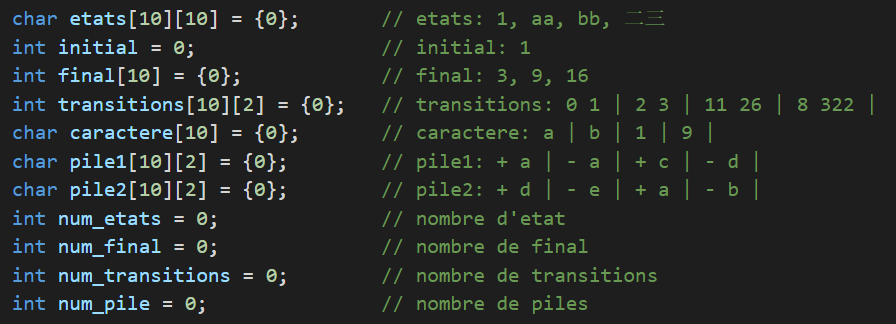
\includegraphics[width=14cm]{analyse_semantique}
			\end{center}
			\caption{Les tableaux et les listes pour enregistrer l'arbre syntaxique correct}
		\end{figure}
		
	\end{itemize}

	\subsection{\textit{compilation}}
	
	\quad Dans cette partie, les cinq fichiers concernés sont \textit{analyseur-lexical.h}, \textit{analyseur-syntaxique.h}, \textit{analyseur-semantique.h}, \textit{compile-automate.h} et \textit{compile-automate.c}. Le *.c fichier contient la \textit{main function} et les *.h fichier contiennent les définitions des fonctions utilisées. Le fichier donné \ doit passer les trois analyses pour qu'il puisse être compilé.
	
	\begin{itemize}
		
		\item 
		Fonction \textit{compilateur} compile l'arbre syntaxique obtenu dans l'analyse sémantique afin d'obtenir la machine virtuelle. La forme de VM est comme suivante:  \par
		
		\begin{figure}[H]
			\setlength{\abovecaptionskip}{-0.cm}
			
			\begin{center}
				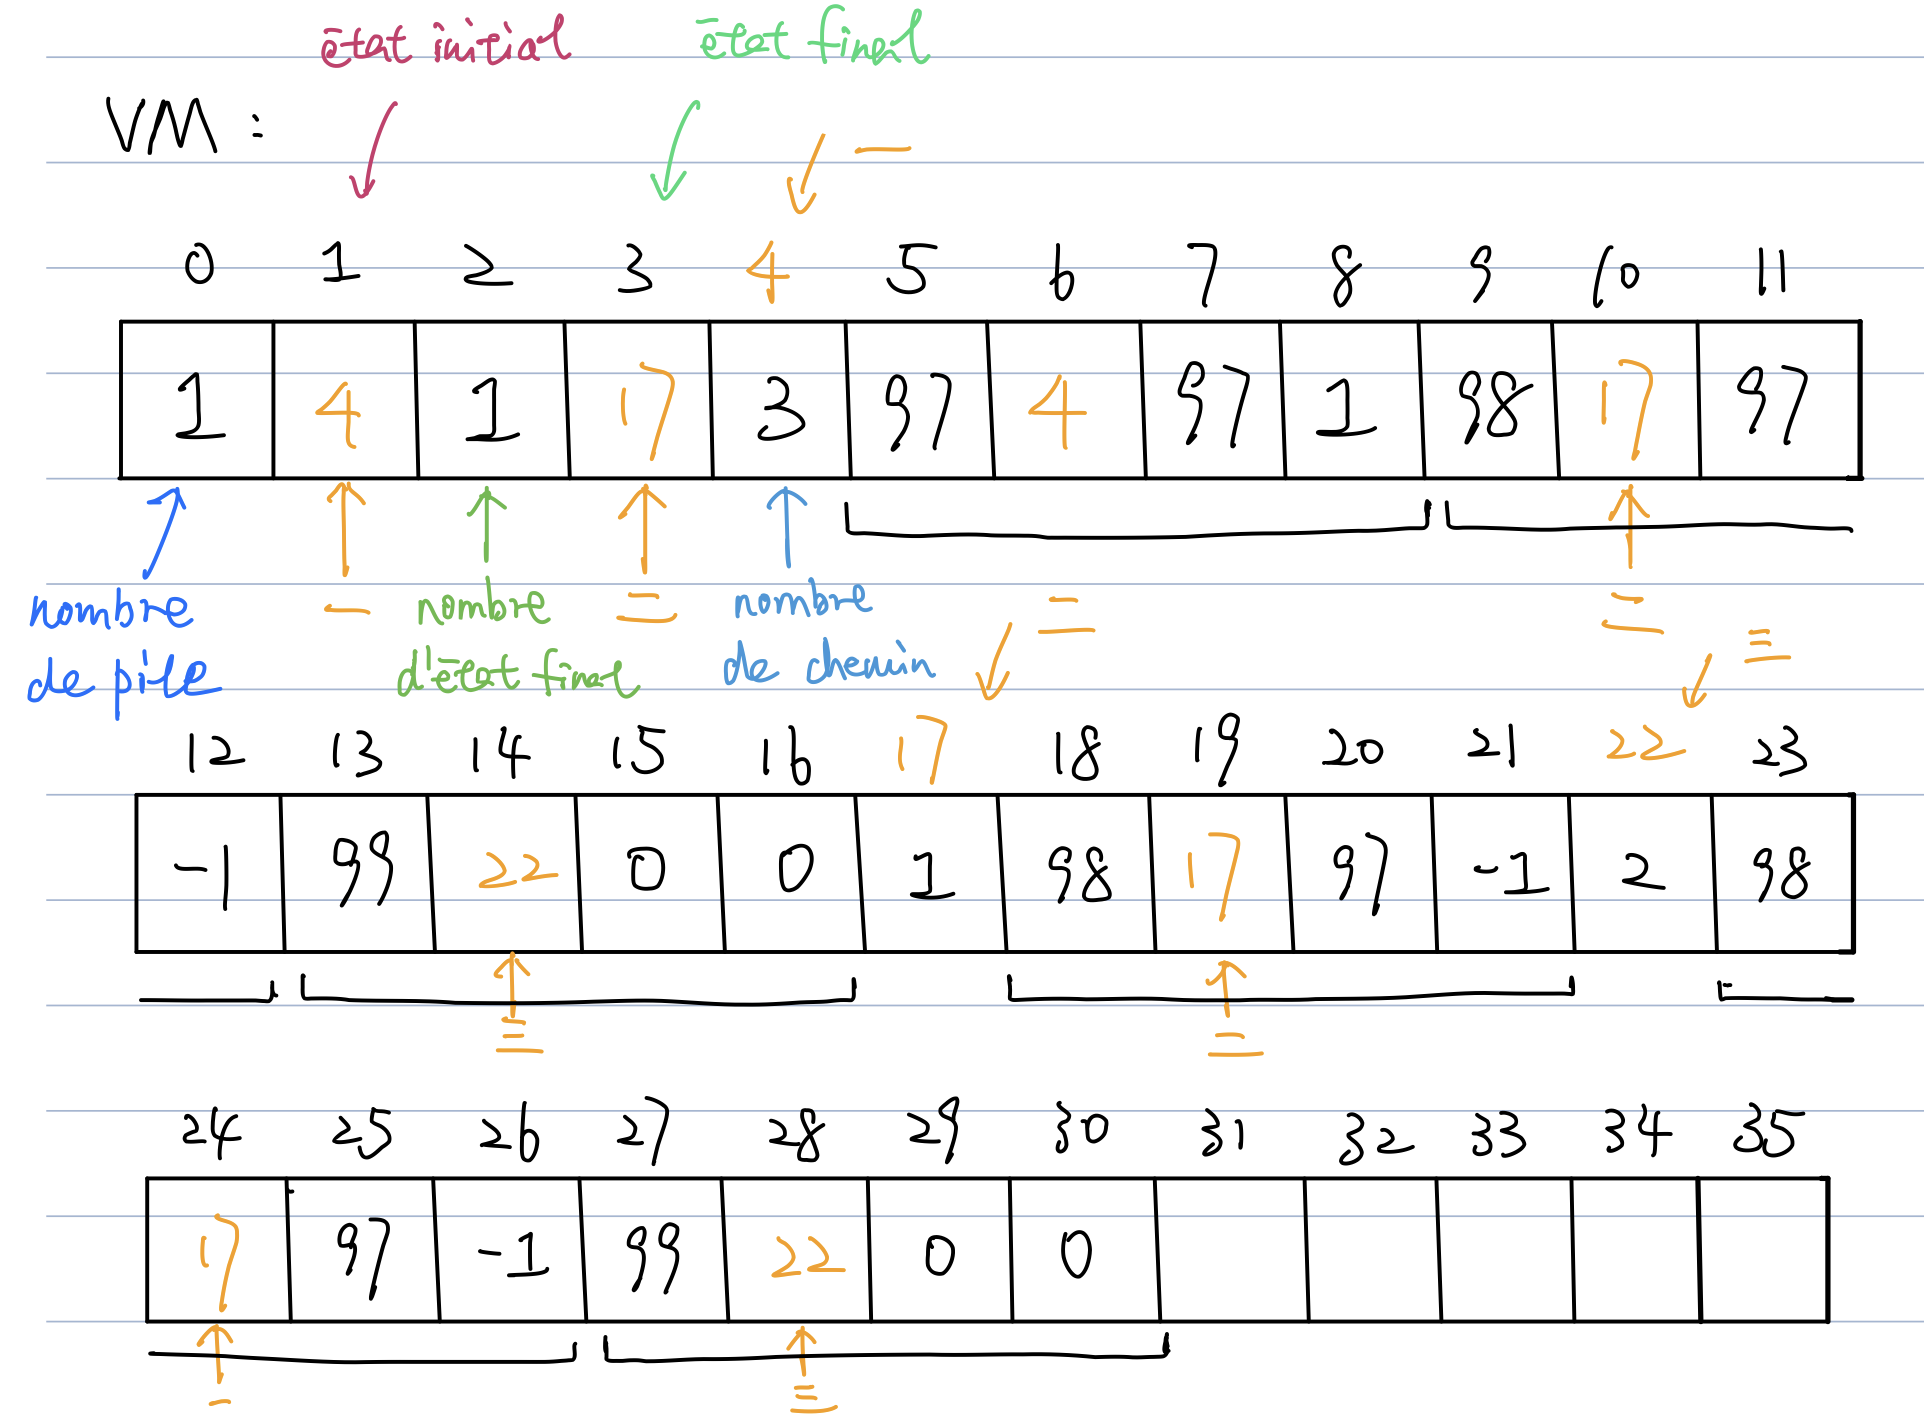
\includegraphics[width=14cm]{vm}
			\end{center}
			\caption{Un exemple de la machine virtuelle avec une pile}
		\end{figure}
	
		\item 
		Fonction \textit{enregistrer-VM} a pour but d'enregister la machine virtuelle dans un fichier. Les sortie de la fonction sont deux fichiers : un fichier \textit{tableau-symbole.txt} contenant des informations des états (noms d'état et leurs addresses dans la VM), et l'autre est le fichier \textit{VM.txt}.  \par
		
	\end{itemize}
	
	\subsection{\textit{exécution}}
	\quad Dans cette partie, les six fichiers concernés sont \textit{analyseur-lexical.h}, \textit{analyseur-syntaxique.h}, \textit{analyseur-semantique.h}, \textit{compile-automate.h}, \textit{executeur.h}et \textit{executeur.c}. Le *.c fichier contient la \textit{main function} et les *.h fichier contiennent les définitions des fonctions utilisées. L'exécuteur prendra le fichier VM et sera capable de reconnaître ou pas un mot saisi au clavier. ll y en a deux modes : \textit{mode normal} et \textit{mode debug}. On va voir comment tester dans la partie suivante.
	  
	\section{Test}
	\quad Dans cette partie, je montre comment "compiler et exécuter" les fichiers que je donnent. Vous pouvez tester avec la même ordre ou comme vous voulez. Je crée trois fichiers avec des erreurs respectivement pour les
	trois analyses. (\textit{Test-lexical.txt, Test-syntaxique.txt et Test-semantique.txt})
	
	\subsection{analyseur-lexical}

	\begin{figure}[H]
		\setlength{\abovecaptionskip}{-0.cm}
		
		\begin{center}
			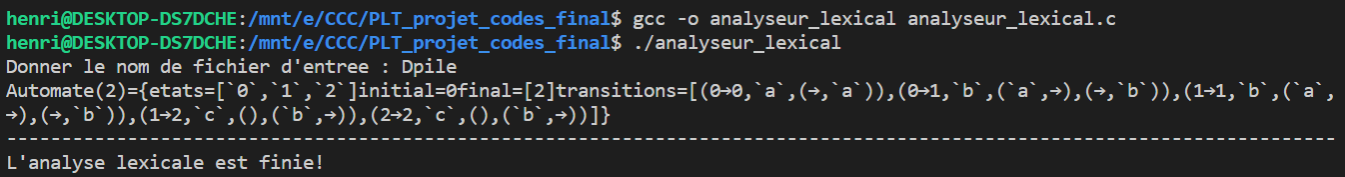
\includegraphics[width=16cm]{lexical1}
		\end{center}
		\caption{Demo: l'analyse lexicale pour Dpile.txt}
	\end{figure}

	\begin{figure}[H]
	\setlength{\abovecaptionskip}{-0.cm}
	
	\begin{center}
		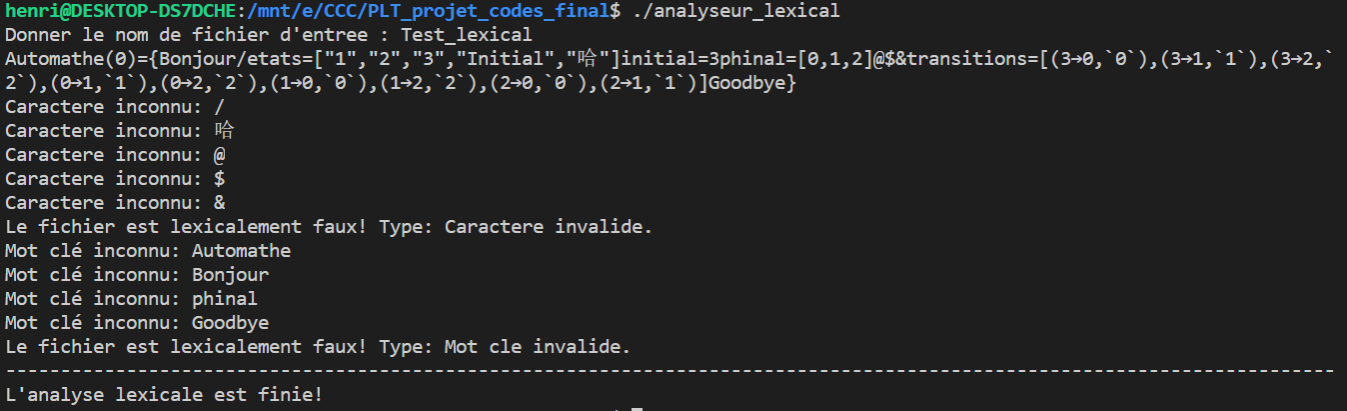
\includegraphics[width=16cm]{lexical2}
	\end{center}
	\caption{Demo: l'analyse lexicale pour Test-lexical.txt}
	\end{figure}

	\subsection{analyseur-syntaxique}
	
	\begin{figure}[H]
		\setlength{\abovecaptionskip}{-0.cm}
		
		\begin{center}
			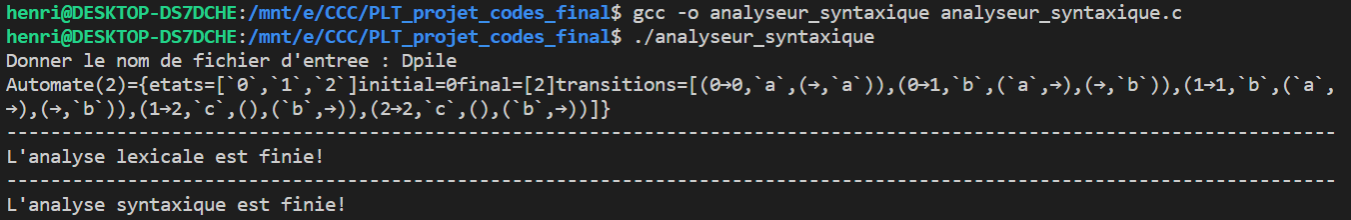
\includegraphics[width=16cm]{syntaxique1}
		\end{center}
		\caption{Demo: l'analyse syntaxique pour Dpile.txt}
	\end{figure}

	\begin{figure}[H]
		\setlength{\abovecaptionskip}{-0.cm}
		
		\begin{center}
			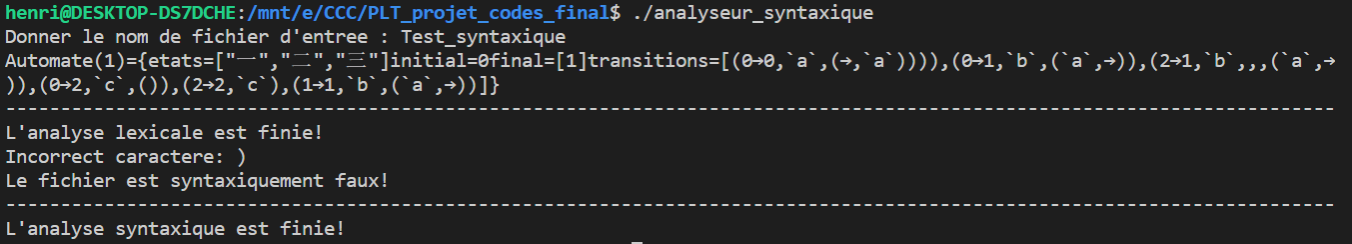
\includegraphics[width=16cm]{syntaxique2}
		\end{center}
		\caption{Demo: l'analyse syntaxique pour Test-syntaxique.txt}
	\end{figure}
	
	\subsection{analyseur-semantique}
	
	\begin{figure}[H]
		\setlength{\abovecaptionskip}{-0.cm}
		
		\begin{center}
			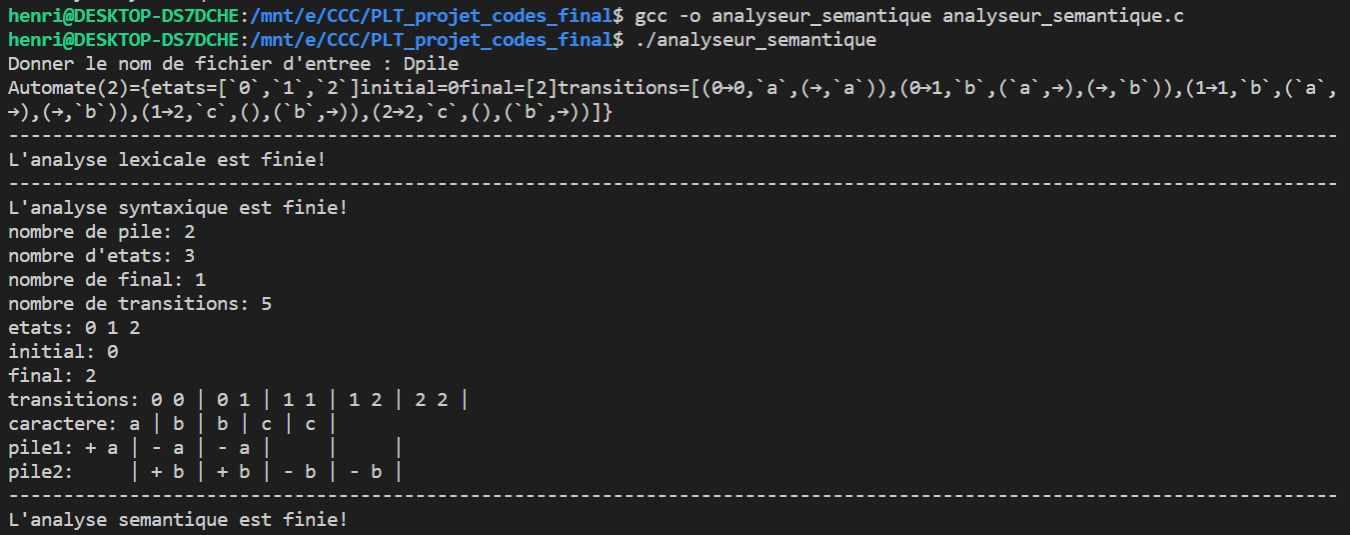
\includegraphics[width=16cm]{semantique1}
		\end{center}
		\caption{Demo: l'analyse sémantique pour Dpile.txt}
	\end{figure}
	
	\begin{figure}[H]
		\setlength{\abovecaptionskip}{-0.cm}
		
		\begin{center}
			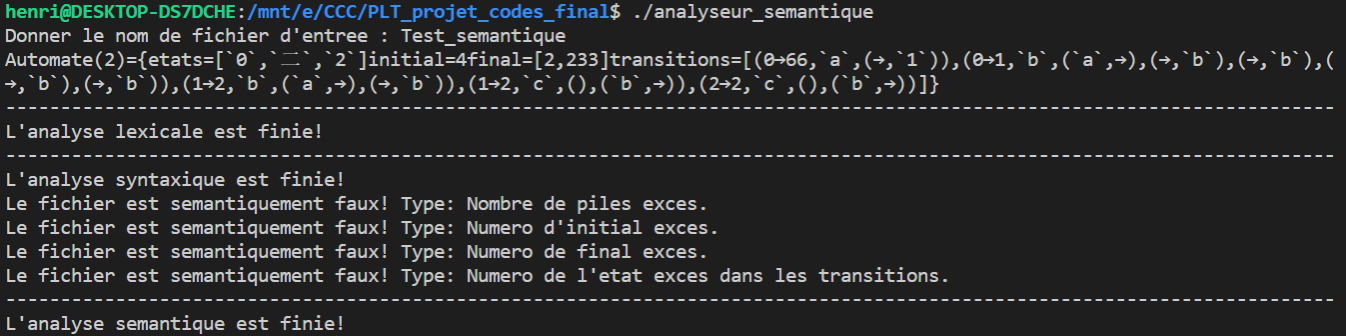
\includegraphics[width=16cm]{semantique2}
		\end{center}
		\caption{Demo: l'analyse sémantique pour Test-semantique.txt}
	\end{figure}
	
	
	\subsection{compile-automate}
	
	\begin{figure}[H]
		\setlength{\abovecaptionskip}{-0.cm}
		
		\begin{center}
			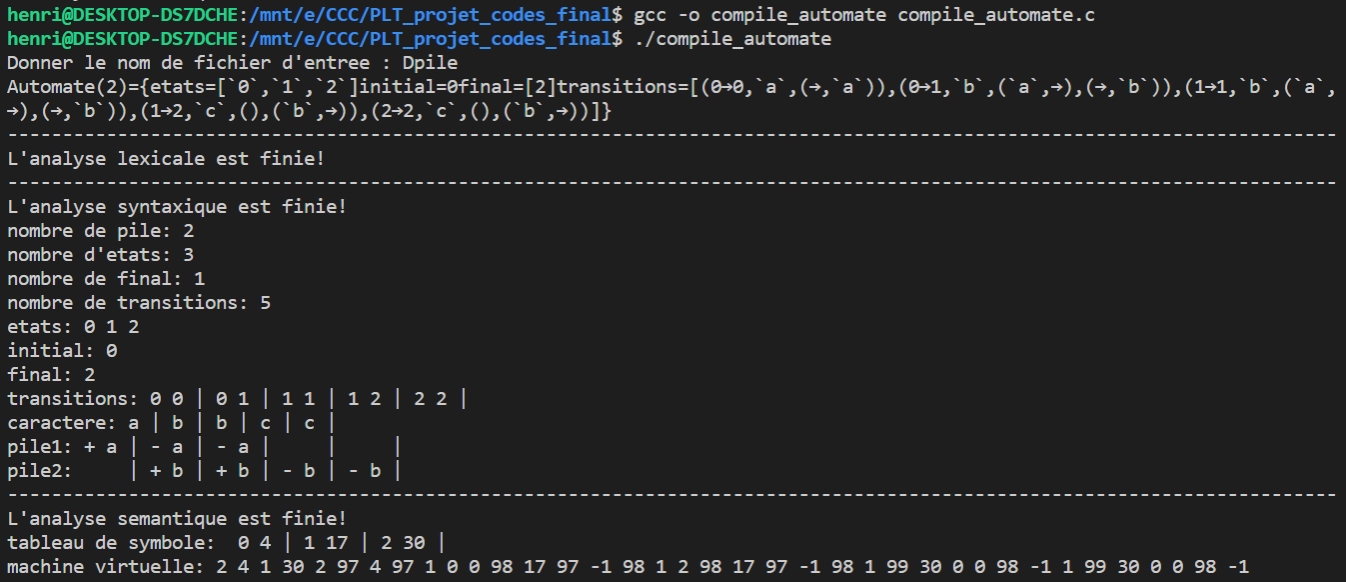
\includegraphics[width=16cm]{compilation1}
		\end{center}
		\caption{Demo: la compilation pour Dpile.txt}
	\end{figure}

	\begin{figure}[H]
	\setlength{\abovecaptionskip}{-0.cm}
	
	\begin{center}
		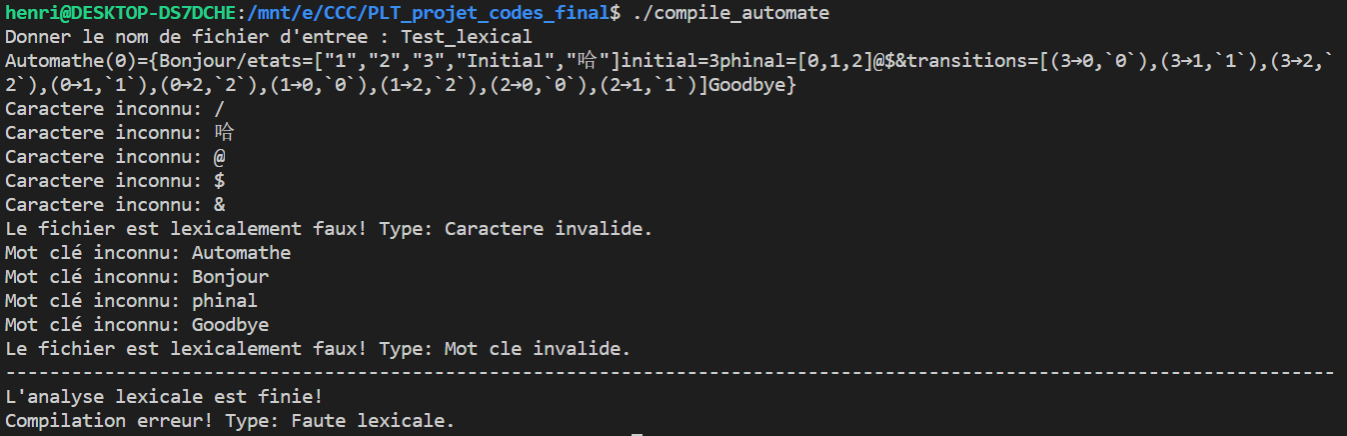
\includegraphics[width=16cm]{compilation2}
	\end{center}
	\caption{Demo: la compilation pour Test-lexical.txt et l'interruption}
	\end{figure}
	
	\subsection{executeur}
	
	\begin{figure}[H]
		\setlength{\abovecaptionskip}{-0.cm}
		
		\begin{center}
			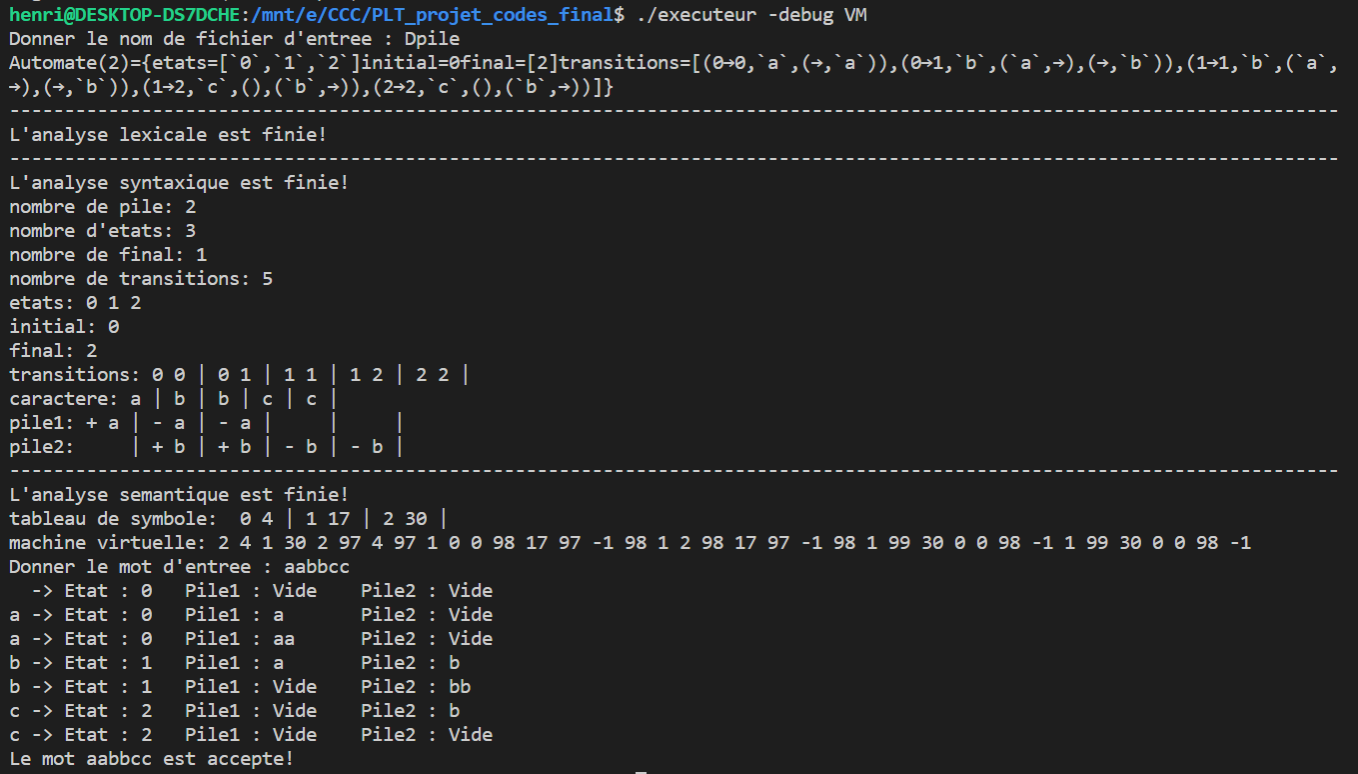
\includegraphics[width=16cm]{executeur1}
		\end{center}
		\caption{Demo: l'exécution pour Dpile.txt et un mot accepté \ dans mode debug}
	\end{figure}

	\begin{figure}[H]
	\setlength{\abovecaptionskip}{-0.cm}
	
	\begin{center}
		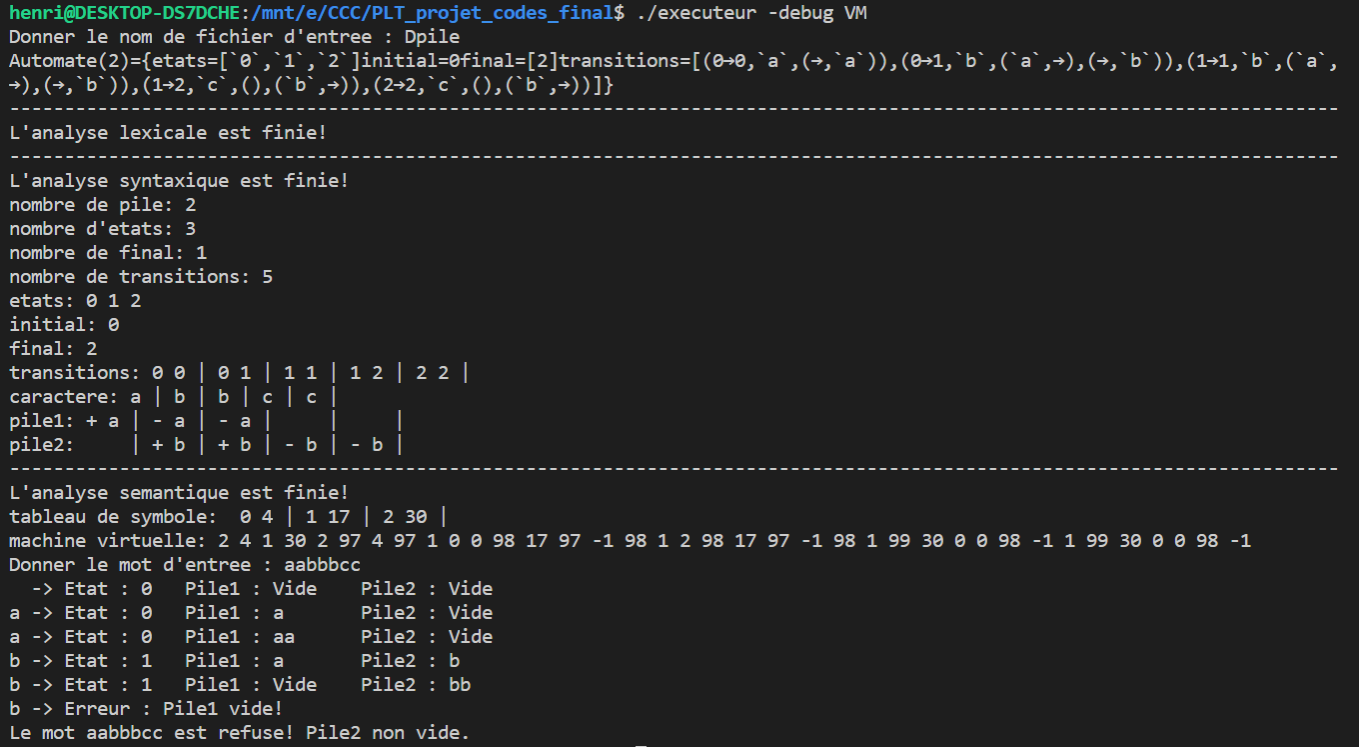
\includegraphics[width=16cm]{executeur2}
	\end{center}
	\caption{Demo: l'exécution pour Dpile.txt et un mot refusé \ dans mode debug}
	\end{figure}

	\begin{figure}[H]
	\setlength{\abovecaptionskip}{-0.cm}
	
	\begin{center}
		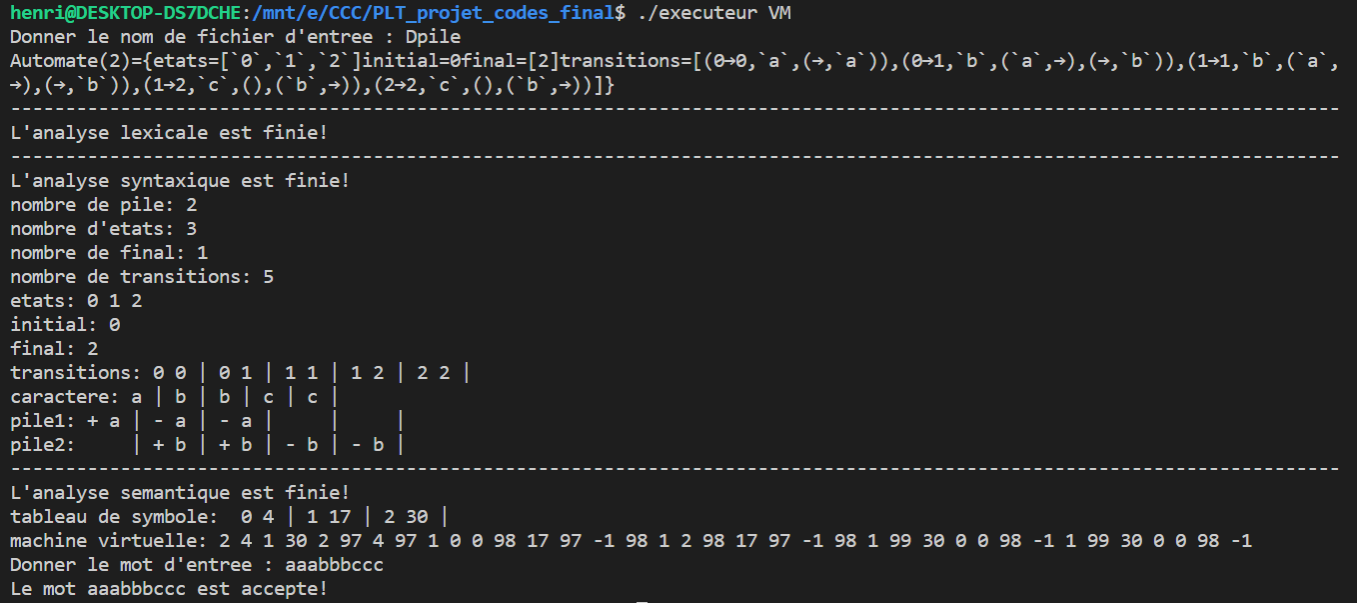
\includegraphics[width=16cm]{executeur3}
	\end{center}
	\caption{Demo: l'exécution pour Dpile.txt dans mode normal}
	\end{figure}

\end{document}